\chapter{Suites et séries de fonctions}
\labch{suites_et_series_de_fonctions}

Le Calcul infinitésimal est l'apprentissage du maniement des \emph{inégalités} bien plus que des égalités, et on pourrait se résumer en trois mots:
\begin{center}
        MAJORER, MINORER, APPROCHER.
\end{center}

V.1 Écart de deux fonctions de \cite{calcul_infinitesimal} \\
De même qu'on cherche à \emph{approcher} un \emph{nombre} inconnu (défini par un procédé quelconque) à l'aide de nombres décimaux (ou rationnels), de même il est naturel en Analyse de chercher à \say{ approcher } une \emph{fonction} complexe inconnue (qui peut être définie par des procédés variés, somme de série, intégrale dépendant d'un paramètre, solution d'équation différentielle, etc.) à l'aide de fonctions que l'on considère comme \emph{connues} (polynômes, fonctions exponentielles, fonctions trigonométriques, etc.). Mais il faut préciser ce qu'on entend par \say{ approcher }, c'est-à-dire \say{ mesurer } en quelque sorte l'\say{ écart } de deux fonctions, de même que la valeur absolue $|x-y|$ mesure l'écart de deux nombres réels ou complexes. \\
L'idée la plus naturelle est que si une fonction $g$ \say{ approche } une fonction $f$ dans un ensemble $E$ où elles sont toutes deux définies, alors, pour chaque $x_0 \in E$, la \emph{valeur} $g(x_0)$ de $g$ doit \emph{approcher} la \emph{valeur} $f(x_0)$ de $f$ au sens usuel, c'est-à-dire que $|f(x_0)-g(x_0)|$ doit être \say{ petit }. Comme ceci doit avoir lieu en \emph{chaque} poit $x_0$ de $E$, on est conduit à prendre pour \say{ écart } de deux fonctions complexes $f$, $g$ définies dans $E$ le nombre
$$d(f, g) = \sup_{x \in E} |f(x)-g(x)|.$$
Lorsqu'il s'agit de fonctions \emph{réelles} $f, g$ définies dans un intervalle $E = [a, b]$ de $\R$, l'idée d'\say{ écart } que nous venons de définir peut se concrétiser graphiquement de la façon suivante: dire que $d(f,g) \leqslant \varepsilon$ signifie que pour tout $x \in E$ on a $g(x)-\varepsilon \leqslant f(x) \leqslant g(x) + \varepsilon$, c'est-à-dire que le graphe de $f$ est \emph{tout entier} contenu dans le \say{ bande } de demi-largeur $\varepsilon$ autour du graphe de $g$. \\
Pour distinguer cette idée d'\say{ approximations } d'autres notions que nous examinerons plus tard \textcolor{red}{à réécrire}, nous dirons qu'il s'agit d'\emph{approximation uniforme} d'une fonction par une autre dans un ensemble $E$ où elles sont toues deux définies; il est important de remarquer que cette notion \emph{dépend essentiellement} de l'ensemble $E$ que l'on considère: si $f$ et $g$ sont toutes deux définies dans un ensemble plus grand $E'$, la relation $|f(x) - g(x)| \leqslant \varepsilon$ pour $x \in E$ n'entraîne nullement $|f(x)-g(x)| \leqslant \varepsilon$ pour $x \in E'$. \\
Étant donnés deux ensembles de fonctions $\mathscr{F}$ (les fonctions \say{ inconnues }) et $\mathscr{G}$ (les fonctions \say{ connues }) toutes définies dans un même ensemble $E$, nous dirons pour abréger qu'\emph{on peut approcher uniformément dans} $E$ les fonctions de $\mathscr{F}$ par les fonctions de $\mathscr{G}$ si, pour toute fonction $f \in \mathscr{F}$ et \emph{tout nombre} $\varepsilon > 0$, il existe une fonction $g \in \mathscr{G}$ (dépendant de $f$ et de $\varepsilon$) telle que l'écart $d(f,g) \leqslant \varepsilon$, c'est-à-dire que 
$$|f(x) - g(x)| \leqslant \varepsilon \quad \text{pour tout } x \in E.$$


\begin{tikzpicture}
    \begin{axis}[width=6.5cm,
        axis lines=middle,
        grid=major,
        xmin=-0.1, xmax=1.1,
        ymin=-0.1, ymax=1.1,
        % xlabel=$x$, xlabel style={right},
        % ylabel=$y$, ylabel style={above},
        tick style={thick},
        ticklabel style={font=\normalsize},
        xtick={0, 1}, 
        ytick={0, 1},
        % legend entries={0.5x},
            legend style={
            at={(1.05,0.4)},
            anchor=north,
            legend columns=1},
            legend cell align={left}
    ]
    
    \def\a{-0.1}
    \def\b{1.1}
    \def\eps{0.5}
    
    \addplot[blue,thick,samples=100,domain=0:\b] {x^3+x-2} {};

    \end{axis}
\end{tikzpicture}

\newpage

\section{Théorème d'approximation de \textsc{Weierstrass}}
Aussi connu sous le nom  de \emph{théorème de \textsc{Stone-Weierstrass}}

\begin{theo}
    Toute fonction continue sur un segment $[a, b]$ de $\R$ à valeurs dans $\R$ ou $\C$ est limite uniforme sur $[a, b]$ d'une suite de polynômes.
\end{theo}

\begin{preuve}
    \cite{calcul_infinitesimal} page 157.
\end{preuve} 

L'exercice suivant montre qu'il existe une suite de polynômes $(P_n)$ qui converge uniformément vers la fonction racine carrée sur $[0, 1]$.

\begin{exercice}
    \emph{Exercice 5. TD Ch. VIII}\\
    Soit la suite de fonctions définie pour tout $x \in [0, 1]$ par
    $$
    \begin{cases}
        P_0(x) &= 0,\\
        P_{n+1}(x) &= P_n (x) + \frac{1}{2} \big( x-P_n (x)^2 \big).
    \end{cases}
    $$
    Montrer que $(P_n)$ converge uniformément vers une fonction $f$ sur $[0, 1]$.
\end{exercice}

\begin{marginfigure}[-5cm]
	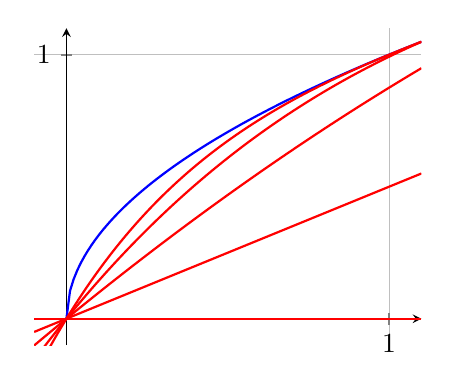
\begin{tikzpicture}
    \begin{axis}[width=6.5cm,
        axis lines=middle,
        grid=major,
        xmin=-0.1, xmax=1.1,
        ymin=-0.1, ymax=1.1,
        % xlabel=$x$, xlabel style={right},
        % ylabel=$y$, ylabel style={above},
        tick style={thick},
        ticklabel style={font=\normalsize},
        xtick={0, 1}, 
        ytick={0, 1},
        % legend entries={0.5x},
            legend style={
            at={(1.05,0.4)},
            anchor=north,
            legend columns=1},
            legend cell align={left}
    ]
    
    \def\a{-0.1}
    \def\b{1.1}
    
    \addplot[blue,thick,samples=100,domain=0:\b] {x^(1/2)} node (racine) {};
    %\node [left] at (racine) {$\sqrt{x}$};
    
    \addplot[red,thick,samples=100,domain=\a:\b] {0} node (P0) {};
    %\node [left] at (P0) {$P_0$};
    
    \addplot[red,thick,samples=100,domain=\a:\b] {x/2} node (P1) {};
    %\node [anchor=north east] at (P1) {$P_1$};
    
    \addplot[red,thick,samples=100,domain=\a:\b] {-1/8*x^2+x} node (P2) {};
    %\node [left] at (P2) {$P_2$};
    
    \addplot[red,thick,samples=100,domain=\a:\b] {-1/128*x^4+1/8*x^3-5/8*x^2+3/2*x} node (P3) {};
    %s\node [left] at (P3) {$P_3$};
    
    \addplot[red,thick,samples=100,domain=\a:\b] {-1/128*x^4+1/8*x^3-5/8*x^2+3/2*x + 1/2*(x-(-1/128*x^4+1/8*x^3-5/8*x^2+3/2*x)^2)} node (P4) {};
    \end{axis}
\end{tikzpicture}


%import matplotlib.pyplot as plt
%import numpy as np
%from numpy.polynomial import Polynomial

%PAS = 1e-3
%n = 8
%X = np.arange(0, 1, PAS)


%P = Polynomial([0])
%plt.plot(X, P(X))

%for k in range(n):
%    P = P + 1/2 * (Polynomial([0, 1]) - P ** 2)
%    plt.plot(X, P(X))

%racine = [np.sqrt(x) for x in X]
%plt.plot(X, racine, 'r')
%plt.show()

\end{marginfigure}

Peut-on génraliser à $\R$ ? \dots

\begin{tcolorbox}
    Si $(P_n)_{n \in \N}$ est une suite de polynômes convergeant uniformément sur $\R$ vers une fonction $f$, alors $f$ est un polynôme.
\end{tcolorbox}

\begin{preuve}
    Source : \cite{exos_oraux} \& \cite{maths-france}. \\
    Soit $(P_n)_{n \in \N}$ une suite de polynômes convergeant uniformément sur $\R$ vers une fonction $f$. \\
    D'après la critère de \textsc{Cauchy} uniforme, il existe un rang $n$ tel que pour tout $p \in \N$, 
    $$\Ninf{P_{n+p} - P_n} \leqslant 1.$$
    La fonction polynomiale $P_{n+p} - P_n$ est donc bornée sur $\R$ autrement dit elle est constante. On a alors,
    $$\forall (p, x) \in \N \times \R,\ P_{n+p}(x) = P_n(x) + P_{n+p}(0) - P_n(0) \xrightarrow[p \to + \infty]{} P_n(x) + f(0) - P_n(0)$$
    donc par unicité de la limite simple, $f : x \mapsto P_n(x) + f(0) - P_n(0)$, qui définit bien une fonction polynomiale. 
\end{preuve}

\section{Approximation polynomiale de \textsc{Bernstein}}
\textsc{Bernstein} a donné une démonstration constructive et probabiliste du théorème de \textsc{Weierstrass} sur $[0, 1]$, en prouvant qu'on pouvait prendre : 

\begin{defi}{Polynôme de \textsc{Bernstein}}
    Le polynôme de \textsc{Bernstein} d'ordre $n$ associé à la fonction $f$ est le polynôme
    \begin{equation} \label{1}
        \Bernstein_n(f)(x) \defeq \sum_{p=0}^{n} f \left( \frac{p}{n} \right) \binom{n}{p} x^p (1-x)^{n-p}
    \end{equation}
\end{defi}

\marginnote[0cm]{Source : \cite{acamanes} \href{https://acamanes.github.io/psi/psi_doc/exos_e08.pdf}{(Exercice 10. TD VIII)}}
\begin{theo}{}
    Soit $f$ une fonction continue sur $I \defeq [0, 1]$. 
    La suite $\big( \Bernstein_n(f) \big)_n$ converge uniformément vers la fonction $f$ sur $I$.
\end{theo}

Nous allons voir deux démonstrations de ce théorème.

\begin{preuve}
    Le démonstration qui suit est celle proposée dans \cite{calcul_infinitesimal} page 159 dont quelques étapes techniques ont été détaillées. \\
    Nous partirons de l'identité
    \begin{equation}
        1 = (1-t+t)^n = \sum_{p=0}^n \binom{n}{p} (1-t)^{n-p}t^p.
    \end{equation}
    On déduit de cette relation que pour toute fonction bornée $f$ définie dans $I$, on a
    \begin{equation} \label{2}
        |\Bernstein_n(f)(t)| \leqslant \sup_{t \in I} |f(t)| \cdot \left(\sum_{p=0}^n \binom{n}{p} (1-t)^{n-p}t^p \right) = d(0, f)
    \end{equation}
    puisque les fonctions $\binom{n}{p}(1-t)^{n-p}t^p$ prennent des \emph{valeurs} $\geqslant 0$ \emph{dans} $I$. \\
    Étant donné $\varepsilon > 0$, on sait que pour toute fonction continue $f$ dans $I$, il existe, en vertu du théorème de \textsc{Weierstrass}, un polynôme $P$ tel que $d(f, P) \leqslant \varepsilon$; on conclut alors de (\ref{2}) que
    \begin{equation} \label{3}
        d(\Bernstein_n(f), \Bernstein_n(P)) \leqslant d(f, P) \leqslant \varepsilon.
    \end{equation}
    Par suite, pour $t \in I$,
    \begin{align*}
        |f(t)-\Bernstein_n(f)(t)| &\leqslant |f(t) - \Bernstein_n(P)(t)| + \underbrace{|\Bernstein_n(P)(t) - \Bernstein_n(f)(t)|}_{\leqslant \varepsilon \text{ d'après (\ref{3})}} \\
        &\leqslant \underbrace{|f(t) - P(t)|}_{\leqslant \varepsilon} + |P(t) - \Bernstein_n(P)(t)| + \varepsilon
    \end{align*}
    Ainsi, par passage à la borne supérieure sur $I$, on obtient
    \begin{equation} \label{5}
        d(f, \Bernstein_n(f)) \leqslant 2 \varepsilon + d(P, \Bernstein_n(P)).
    \end{equation}
    Si l'on prouve le théorème lorsque $f$ est un \emph{polynôme}, il sera donc vrai pour toute fonction continue dans $I$. Par linéarité, il suffit donc de le prouver lorsque $f(t) = t^m$. En fait, nous allons voir, par récurrence sur $m$, que l'on a, en posant $f_m(t) = t^m$, pour $n \geqslant m$, 
    \begin{equation} \label{6}
        \Bernstein_n(f_m)(t) = t^m + \frac{1}{n}Q_{m,n}(t)
    \end{equation}
    où $Q_{m,n}$ est un polynôme de degré inférieur à $m-1$, dont les coefficients sont majorés en valeur absolue par un nombre $A_m$ \emph{indépendant de} $n$. \\
    La formule (\ref{6}) se réduit à (\ref{2}) pour $m=0$, avec $Q_{0,n}(t) = 0$. Supposons-la vérifiée pour un entier $m$ et dérivons par rapport à $t$; en vertu de la défition (\ref{1}), on obtient, pour $n \geqslant m+1$, 
    \begin{equation} \label{7}
        -\sum_{p=0}^{n-1} \binom{n}{p} \frac{p^m}{n^m}(n-p)(1-t)^{n-p-1}t^p + \sum_{p=1}^n \binom{n}{p} \frac{p^{m+1}}{n^m}(1-t)^{n-p}t^{p-1} = mt^{m-1} + \frac{1}{n} Q'_{m,n}(t).
    \end{equation}
    Comme $(n-p) \binom{n}{p} = n \binom{n-1}{p}$, le premier terme du premier membre de (\ref{7}) est égal à 
    $$-n \Bernstein_{n-1}(f_m)(t) = -nt^m - \frac{n}{n-1}Q_{m, n-1}(t).$$ 
    Multipliant les deux membres de (\ref{7}) par $\frac{t}{m}$, on obtient donc, en vertu de la définition des polynômes de \textsc{Bernstein},
    \begin{equation*}
        -\frac{n}{m} t^{m+1} - \frac{nt}{m(n-1)}Q_{m, n-1}(t) + \frac{n}{m} \underbrace{\sum_{p=1}^n \binom{n}{p} \frac{p^{m+1}}{n^{m+1}}(1-t)^{n-p}t^p}_{\Bernstein_n(f_{m+1})(t)} = t^m + \frac{t}{mn}Q'_{m,n}(t)\\
    \end{equation*}
    soit en réarrangeant les termes et en multipliant l'égalité par $\frac{m}{n}$;
    \begin{align*}
        \Bernstein_n(f_{m+1})(t) &= t^{m+1} + \frac{m}{n}t^m + \frac{t}{n^2}Q'_{m,n}(t) + \frac{t}{n-1} Q_{m, n-1}(t) \\
        &= t^{m+1} + \frac{1}{n}Q_{m+1, n}(t)
    \end{align*}
    avec $Q_{m+1, n}(t) = mt^m + \frac{1}{n}t Q'_{m,n}(t) + \frac{n}{n-1}t Q_{m,n-1}(t)$. \\
    Comme, par hypothèse, $Q_{m,n}$ est de degré inférieur à $m-1$, le polynôme $Q_{m+1, n}$ est bien de degré inférieur à $m$. \\
    Les coefficients de $\frac{1}{n}t Q'_{m,n}(t)$ sont majorés en valeur absolue par $\frac{m-1}{n}A_m \leqslant (m-1)A_m$ ... \textcolor{red}{A FINIR}
    et cela prouve (\ref{6}) par récurrence, avec
    $$A_{m+1} \leqslant 3 \sup(m, (m-1) A_m).$$
\end{preuve}

Le sujet \textsc{x/ens psi 2018} propose une démonstration élégante de ce résultat d'analyse pure en passant par les probabilités. (Je crois que la version du TD est un peu différente).
Préciser les hypothèses sur $f$.
\begin{exercice}        
    Soit $x \in ]0, 1[$ et $n \in \Ne$. On considère $X_1, \dots, X_n$ des variables aléatoires mutuellement indépendantes et suivant toutes la même loi de \textsc{Bernoulli} de paramètre $x$. On pose
    $$S_n = \frac{X_1 + \cdots + X_n}{n}.$$
    \begin{enumerate}
        \item Exprimer $\E(S_n)$, $\V(S_n)$ et $\E(f(S_n))$ en fonction de $x$, $n$ et du polynôme $\Bernstein_n(f)$.
        \item En déduire les inégalités:
        $$\sum_{k=0}^{n} \left| x- \frac{k}{n} \right| \binom{n}{k} x^k (1-x)^{n-k} \leqslant \V(S_n)^{1/2} \leqslant \frac{1}{2\sqrt{n}}.$$
        \item Montrer que $\lambda^\alpha \leqslant 1+\lambda$ pour tout réel $\lambda > 0$ et en déduire l'inégalité:
        $$\left|x-\frac{k}{n} \right|^\alpha \leqslant n^{-\alpha/2} \Bigg(1 + \sqrt{n} \left|x - \frac{k}{n} \right| \Bigg)$$
        pour tout $x \in ]0, 1[, n \in \Ne$ et $k \in \llbracket 1, n \rrbracket$.
        \item Soit $n \in \Ne$. Montrer que 
        $$\Ninf{f-\Bernstein_n(f)} \leqslant \frac{3k}{2} \frac{1}{n^{\alpha/2}}.$$
        Conclure.
    \end{enumerate}
\end{exercice}

\marginnote[0cm]{
    \begin{prop}{\note Somme de \textsc{Bernoulli} indépendantes}
        La somme de $n$ variables aléatoires discrètes indépendantes suivant la même loi de \textsc{Bernoulli} de paramètre $p$ suit une loi binomiale de paramètres $(n, p)$. 
    \end{prop}
    La démontration est immédiate en passant par les fonctions génératrices.
}

\begin{preuve}
    Soit $x \in [0, 1]$. On considère une suite de variables aléatoires $(X_n)_n$ indépendantes identiquement distribuées de loi de \textsc{Bernoulli} $\mathscr{B}(x)$. Ainsi, $S_n \defeq \sum\limits_{i=1}^n X_i$ suit une loi binomiale $\mathscr{B}(n, x)$ \note et par le théorème de transfert
    $$\E \left[ f\left( \frac{S_n}{n} \right) \right] = \sum_{p=0}^n \binom{n}{p} f \left( \frac{p}{n} \right) (1-x)^{n-p} x^p = \Bernstein_n(f)(x).$$
    On va chercher à utiliser la convergence en probabilité de $\frac{S_n}{n}$ vers $x$. \\
    Soit $\varepsilon > 0$. La fonction $f$ étant continue sur le compact $[0, 1]$ donc d'après le théorème de \textsc{Heine} \note, elle y est uniformément continue i.e.
    $$\exists \eta > 0, |x-y| \leqslant \eta \Rightarrow |f(x) - f(y)| \leqslant \varepsilon.$$
    \marginnote[-4cm]{
        \begin{theo}{\note Théorème de \textsc{Heine}}
             Une fonction continue sur un segment, plus généralement sur un compact, y est uniformément continue. 
        \end{theo}
    }
    On va alors scinder en deux. On a
    \marginnote[0cm]{On retrouve cette méthode de séparation avec la fonction indicatrice dans la démonstration de l'inégalité de \textsc{Markov}.}
    \begin{align*}
        |f(x) - \Bernstein_n(f)(x)| &= \left| \E \left[ f(x) - f\left( \frac{S_n}{n} \right) \right] \right| \leqslant \E \left[ \left| f(x) - f \left( \frac{S_n}{n} \right) \right| \right] \\
        &\leqslant \E \left[ \left| f(x) - f \left( \frac{S_n}{n} \right) \right| \mathds{1}_{\left| x - \frac{S_n}{n} \right| < \eta} + \left| f(x) - f \left( \frac{S_n}{n} \right) \right| \mathds{1}_{\left| x - \frac{S_n}{n} \right| \geqslant \eta} \right] \\
        \text{par linéarité de l'espérance } &\leqslant \E \left[ \left| f(x) - f \left( \frac{S_n}{n} \right) \right| \mathds{1}_{\left| x - \frac{S_n}{n} \right| < \eta} \right] + \E \left[ \left| f(x) - f \left( \frac{S_n}{n} \right) \right| \mathds{1}_{\left| x - \frac{S_n}{n} \right| \geqslant \eta} \right] \\
        &\leqslant \varepsilon + 2 \Ninf{f} \E \left[ \mathds{1}_{\left| x - \frac{S_n}{n} \right| \geqslant \eta} \right] \\
        \text{par l'espérance d'une indicatrice } &\leqslant \varepsilon + 2 \Ninf{f} \P \left( \left| x - \frac{S_n}{n} \right| \geqslant \eta \right).
    \end{align*}
    On utilise alors l'inégalité de \textsc{Bienaymé}-\textsc{Tchebychev} \note (on rappelle que $\E[S_n/n] = x$)
    \marginnote[-2cm]{
        \begin{theo}{\note Inégalité de \textsc{Bienaymé}-\textsc{Tchebychev}}
            Soit $X$ une v.a.r.d. admettant un moment d'ordre $2$,
            $$\forall \varepsilon > 0,\ \P \big(|X-\E[X]| \geqslant \varepsilon \big) \leqslant \frac{\V(X)}{\varepsilon^2}.$$
        \end{theo}
    }
    \begin{align*}
        |f(x) - \Bernstein_n(f)(x)| &\leqslant \varepsilon + 2 \Ninf{f} \frac{\V(S_n/n)}{\eta^2} \\
        &\leqslant \varepsilon + 2 \Ninf{f} \frac{\V(S_n)}{n^2 \eta^2} \\
        &\leqslant \varepsilon + 2 \Ninf{f} \frac{x(1-x)}{n \eta^2} \\
        &\leqslant \varepsilon + \Ninf{f} \frac{1}{2 n \eta^2} \text{ indépendant de $x$}.
    \end{align*}
    Ainsi, on a $\lim \sup_n \Ninf{f - \Bernstein_n(f)} \leqslant \varepsilon$, et on a en faisant tendre $\varepsilon$ vers $0$:
    $$\Ninf{f - \Bernstein_n(f)} \xrightarrow[n \to + \infty]{} 0.$$
\end{preuve}

\begin{remarque}
    Ce résultat peut être étendu à toute fonction continue sur un segment $[a, b]$ en posant
    $$\forall x \in [0, 1], f(x) = g \big( (b-a)x + a \big).$$
    La fonction $x \mapsto (b-a)x + a$ est un homéomorphisme de $[0, 1]$ sur $[a, b]$.
\end{remarque}

\section{Intégration d'une série de fonctions}
Soit $S:x \to \sum\limits_{n=1}^{+\infty} \frac{(-1)^n}{1+n^2 x^2}$.
\begin{itemize}
    \item Donner l'ensemble de définition de $S$ et donner un équivalent en $+\infty$.\\
    $\blacktriangleright$  $D_S = \Re$.\\
    $\blacktriangleright$ On se doute que $S$ \textbf{se comporte comme} $\frac{1}{x^2}$ en $+\infty$. L'idée est donc de déterminer la limite de $x^2 S(x)$ en $+\infty$. Le \textbf{théorème d'interversion des limites} permet d'affirmer que cette limite est finie et qu'elle est égale à $c = \sum\limits_{n=1}^{+\infty} \frac{(-1)^n}{n^2}$. Une séparation des termes pairs et impairs de la somme (et le résultat du \href{https://fr.wikipedia.org/wiki/Problème_de_Bâle}{problème de Bâle}) permet de montrer que $c = -\frac{\pi^2}{12}$ et donc $S(x) \sim_{+\infty} -\frac{\pi^2}{12x^2}$.
    \item Montrer que $S$ est intégrable sur $\Rpe$ et calculer $\int_0^{+\infty} S(t) \mathrm{d}t$.\\
    $\blacktriangleright$ Comme $S$ est une série alternée, on peut lui appliquer le \textbf{théorème des séries alternées} et écrire que 
    $$|S(x)| \leqslant \frac{1}{1+x^2} \text{ (majoration du reste d'ordre 1)}$$
    L'intégrabilité du majorant sur $\Rpe$ assure celle de $S$ sur cet ensemble. \textcolor{green}{Est-ce que l'intégrabilité sur R+* des termes de la somme et leur CU vers $S$ impliquent l'ingrabilité de $S$ sur cet ensemble ? c.f. théorème de la convergence dominée peut-être...}\\
    $\blacktriangleright$ L'interversion série/intégrale permet de montrer que $\int_0^{+\infty} S(t) \d t = \frac{\pi}{2} \sum\limits_{n=1}^{+\infty} \frac{(-1)^n}{n} = -\frac{\pi}{2} \ln(2)$ (c.f. \nameref{deux_sommes}).\\
    \textcolor{green}{Dans la correction (p. 374), on effectue le calcul sur une somme partielle et on détermine ensuite la limite de cette somme. J'avais naïvement travailler avec l'intégrale jusqu'en +infini et la somme aussi, \textbf{est-ce licite ?}}.
\end{itemize}

\section{Équivalent d'une série de fonctions}
\begin{exercice}
    On pose $f(x) = \sum\limits_{n=1}^{+\infty}\frac{x}{n(1+nx^2)}$. Donner un équivalent de $f$ et $0^+$.
\end{exercice}

\begin{solution}
    Éffectuer une comparaison série/intégrale aux termes de la somme pour encadrer $f$ (ne pas oublier de justifier l'intégrabilité des fonctions sur $[1, +\infty[$):
    $$\int_{2}^{+\infty} \frac{x}{t(1+tx^2)} \d t + \frac{x}{1+x^2} \leqslant f(x) \leqslant \int_{1}^{+\infty} \frac{x}{t(1+tx^2)} \d t + \frac{x}{1+x^2}.$$ 
    Décomposer les intégrandes en éléments simples et calculer les intégrales:
    $$-2x \ln(x) + o_0(x\ln(x)) \leqslant f(x) \leqslant -2x \ln(x) + o_0(x\ln(x))$$
    Finalement, 
    $$f(x) \isEquivTo{0^+} -2x\ln(x)$$
\end{solution}

\section{Série de fonctions continues dont la somme est discontinue}
\begin{prop}{}
    \marginnote[0cm]{Source : \cite{contre-exemples} p.257}
    Soit la suite $(f_n)_{n \geqslant 0}$ d'applications continues de $[0,1]$ dans $\R$, de terme général
    \begin{alignat*}{2}
        f_n\ :\ [0,1]\ &\longrightarrow\ \R\\
        x\ &\longmapsto\ f_n(x) = (1-x)x^n.
    \end{alignat*}
    La somme des $f_n$ est discontinue.
\end{prop}

\begin{preuve}
    Pour tout point $x$ de $[0,1[$, la série $\sum f_n(x)$ est le produit par $(1-x)$ d'une série géométrique de raison $x$ où $0 \leqslant x < 1$, donc elle converge et sa somme est égale à $(1-x)/(1-x) = 1$. De plus $f_n(1) = 0$ pour tout entier naturel $n$. La série de fonctions $\sum f_n$ converge donc simplement sur le segment $[0,1]$ et sa somme est l'application 
    \begin{alignat*}{2}
        S\ :\ [0,1]\ &\longrightarrow\ \R\\
        x\ &\longmapsto\ S(x) =
        \begin{cases}
            1 &\text{ si } x \in [0,1[,\\
            0 &\text{ si } x = 1,
        \end{cases}
    \end{alignat*}
    qui est discontinue en $1$.
\end{preuve}


\section{Fonction \texorpdfstring{$\zeta$}{zêta} alternée}
\marginnote[0cm]{Source : \cite{acamanes} \href{https://acamanes.github.io/psi/psi_doc/exos_e08.pdf}{(Exercice 13. TD VIII)}}
On définit la fonction $\zeta$ alternée $F$ comme suit
$$F(x) = \sum_{n=1}^{+ \infty} \frac{(-1)^{n-1}}{n^x}.$$
\begin{itemize}
    \item Déterminer l'ensemble de défintion de $F$ et trouver une relation entre $F$ et $\zeta$.
    \begin{itemize}
        \item Calculer $\zeta(x) - F(x)$ pour trouver que $\zeta(x) = \frac{1}{1-2^{1-x}} F(x)$.
    \end{itemize}
    \item Déterminer $\displaystyle \lim_{x \to 1} (x-1) \zeta(x)$.
    \begin{itemize}
        \item En comparant $\zeta$ à une intégrale, on peut montrer que $\frac{1}{1-x} \leqslant \zeta(x) \leqslant \frac{1}{1-x} + 1$.
    \end{itemize}
    \item On peut aussi procéder de la manière suivante: $\zeta$ est décroissante sur $]1, +\infty[$ donc $\zeta$ admet une limite $\ell \in \Rp \cup \{ + \infty \}$ en $1$.\\
        $\blacktriangleright$ Si $\ell \in \Rp$, par passage à la limite dans l'inégalité $\zeta(x) \geqslant \sum\limits_{n=1}^{N} \frac{1}{n^x}$, $$\ell \geqslant \sum\limits_{n=1}^{N} \frac{1}{n} \xrightarrow[N \to + \infty]{} +\infty.$$ 
        Donc $\ell = + \infty$ et $\displaystyle \lim_{x \to 1} \zeta(x) = +\infty$. 
    \item Déterminer $\displaystyle \lim_{x \to +\infty} F(x)$ ainsi qu'un équivalent de $\zeta$ en $+\infty$.
    \begin{itemize}
        \item On peut montrer que (\textcolor{green}{à détailler}) $\zeta(x) \sim_{+ \infty} 1$.
    \end{itemize}
\end{itemize}

\section{Fonctions continues nulle part dérivables}
\marginnote[0cm]{
\emph{\say{ Je me détourne avec effroi et horreur de cette plaie lamentable des fonctions continues qui n'ont point de dérivées. }} \\
\hspace*{\fill} Charles \textsc{Hermite} (1893) \\
\emph{\say{ C’est un cas où il est vraiment naturel de penser à ces fonctions continues sans dérivées que les mathématiciens ont imaginées, et que l’on regardait à tort comme de
simples curiosités mathématiques, puisque l’expérience peut les suggérer. }} \\
\hspace*{\fill} Jean \textsc{Perrin} \sidenote{Physicien, chimiste et homme politique français (1870 - 1942), prix Nobel de physique 1926.}, au sujet du mouvement brownien.
}

\cite{contre-exemples} p. 160 \\
Jusqu'à la moitié du \textsc{xix}$^\me$ siècle, on pensait généralement qu'une fonction continue était dérivable sauf peut-être en quelques points. \textsc{Ampère} prétendit même l'avoir démontré en 1806. \textsc{Bolzano} donne vers 1830 un exemple de fonction continue, mais dérivable nulle part; cependant ses écrits restent méconnus. En 1854, Bernhard \textsc{Riemann}, propose sans preuve, la fonction:
$$R:x \mapsto R(x) \defeq \sum_{n=1}^{+\infty} \frac{\sin(n^2 x)}{n^2}.$$
Karl \textsc{Weierstrass} se déclare incapable de la démontrer. Il faut attendre 1971 pour savoir que $R$ n'est pas dérivable sauf en certains points. En 1872, Karl \textsc{Weierstrass} démontre que si $a$ et $b$ sont des réels tels que $a > 0$, $b > 0$ et $ab > 1 + \frac{3 \pi}{2}$, la fonction:
$$f : x \mapsto f(x) \defeq \sum_{n=1}^{+\infty} b^n \cos(a^n x)$$
est continue sur $\R$ et n'est dérivable en aucun point de $\R$.

\textbf{Notations.}\\
On note $E$ l'ensemble des fonctions continues sur $[0, 1]$ et $F$ l'ensemble des fonctions continues sur $[0, 1]$, nulle part dérivables sur $[0, 1]$. 

\begin{theo}{}
    L'ensemble $F$ est non vide.
\end{theo}

\begin{preuve}
    \marginnote[0cm]{\url{https://share.miple.co/content/XEZ7y9BayeSN1}}
    Notons:
    \begin{itemize}
        \item $\forall x \in \Rp, \Delta(x) \defeq \min\limits_{n \in \N} |x - n|$,
        \item $\forall x \in \Rp, \Delta_n(x) \defeq \frac{\Delta(2^n x)}{2^n x}$,
        \item $\forall x \in [0, 1], W(x) \defeq \sum\limits_{n=0}^\infty \Delta_n(x)$.
    \end{itemize}
    Nous allons montrer que la fonction $W$ est un élément de $F$.
    \begin{itemize}
    \item[$\rhd$] \textbf{Continuité.} La fonction $\Delta$ est minimale sur $\N$ où elle vaut $0$, et est maximale sur $\N + \frac{1}{2}$ où elle vaut $\frac{1}{2}$, d'où $\Ninf{\Delta} \leqslant \frac{1}{2}$ et donc $\Ninf{\Delta_n} \leqslant \frac{1}{2^{n+1}}$. Les fonction $\Delta_n$ étant continues et $\sum \Delta_n$ convergeant normalement, la fonction $W$ est continue. 
    \item[$\rhd$] \textbf{Non-dérivabilité.} Soit $x \in [0, 1]$. On note, pour tout $p \in \N$, 
    $$x_p \defeq \frac{\lfloor 2^p x \rfloor}{2^p} \text{ et } y_p \defeq x_p + \frac{1}{2^p}.$$ 
    Étudions la limite de $\limits \frac{W(x_p) - W(y_p)}{x_p - y_p}$ quand $p$ tend vers $+ \infty$:
    \begin{itemize}
        \item Si $n \geqslant p$, alors $2^n x_p$ et $2^n y_p$ sont des entiers. Donc $\Delta_n(x_p) = \Delta_n(y_p) = 0$ et $\frac{\Delta_n(x_p) - \Delta_n(y_p)}{x_p - y_p} = 0$.
        \item Si $n < p$, alors $x_p, y_p \in I_1 \defeq \left[ x_n, \frac{x_n + y_n}{2} \right]$ ou $x_p, y_p \in I_2 \defeq \left[ \frac{x_n + y_n}{2}, y_n \right]$. $\Delta_n$ a une pente $1$ sur $I_1$ et une pente $-1$ sur $I_2$. Donc $\frac{\Delta_n(x_p) - \Delta_n(y_p)}{x_p - y_p} = (-1)^{\lfloor 2^{n+1} x \rfloor}$. 
    \end{itemize}
    Donc:
    $$\frac{W(x_p) - W(y_p)}{x_p - y_p} = \sum_{n=0}^{p-1} (-1)^{\lfloor 2^{n+1} x \rfloor}.$$
    Notons $r_p \defeq \frac{W(y_p) - W(x_p)}{y_p - x_p}$. La suite $(r_p)_{p \in \N}$ ne converge par puisque $r_{p+1} - r_p = (-1)^{\lfloor 2^{n+1} x \rfloor}$ ne tend pas vers $0$. \\
    Comme $x_p \xrightarrow[p \to \infty]{} x$ et $y_p \xrightarrow[p \to \infty]{} x$, on en conclut que $W$ n'est pas dérivable en $x$ et donc est nulle part dérivable sur $[0, 1]$.
    \end{itemize}
\end{preuve}

\subsection{Courbe du blancmanger ou de \textsc{Takagi}}

\marginnote[0cm]{\cite{contre-exemples} p. 160}
En 1903, le mathématicien japonais Teiji \textsc{Takagi} (1875-1960) propose les fonctions:
$$f : x \mapsto f(x) \defeq \sum_{n=0}^{+ \infty} b^n g(a^n x)$$
où $g$ est la fonction de $g : x \mapsto d(x, \Z)$ (distance de $x$ à $\Z$) de $\R$ dans $\R$ et $a$ et $b$ des réels tels que $0 < b < 1$ et $a \leqslant 4$. Lorsque de plus $ab > 2$, la fonction $f$ a des dérivées supérieures égales à $+\infty$ et inférieures égales à $- \infty$ en tout point de $\R$. \\

\marginnote[0cm]{Alain \textsc{Camanes} DS MPSI1 10/01/2015}
La fonction de \textsc{Takagi} a été introduite par Teiji \textsc{Takagi} en 1903 motivé par les fonctions nulle part dérivables de \textsc{Weierstrass} après une visite en Allemagne de 1897 à 1901. \\
Une variante de la fonction de \textsc{Takagi}, utilisant la base $10$ et non la base $2$, a été introduite par \textsc{Van der Waerden} en  1930. Bien que non différentiables, ces fonctions possèdent des dérivées infinies en de nombreux points (tout comme la fonction de \textsc{Weierstrass}). C'est pourquoi \textsc{Knopp} a introduit en 1918 une variante de la fonction de \textsc{Takagi} qui, en tout point, n'admet ni de dérivée finie ni de dérivée infinie.

\begin{figure*}[h!]
    \centering
    \begin{tikzpicture}[scale=0.8]

    \begin{scope}[local bounding box=struct, scale=3]
        \draw[red] (0, 0) -- (1/2, 1/2) -- (1, 0);
    \end{scope}
    
    \begin{scope}[shift={($(struct.east)+(1,-3/4)$)}, scale=3]
        \draw[dashed] (1/4, 1/4) -- (1/2, 1/2) -- (3/4, 1/4);
        \draw[red] (0, 0) -- (1/4, 1/4) -- (1/2, 0) -- (3/4, 1/4) -- (1, 0);
        \draw (0, 0) -- (1/4, 1/2) -- (3/4, 1/2) -- (1, 0);
    \end{scope}
    
    \begin{scope}[shift={($(struct.east)+(5,-3/4)$)}, scale=3]
        \draw[dashed] (0, 0) -- (1/4, 1/2) -- (3/4, 1/2) -- (1, 0);
        \draw[red] (0, 0) -- (1/8, 1/8) -- (1/4, 0) -- (3/8, 1/8) -- (1/2, 0) -- (5/8, 1/8) -- (6/8, 0) -- (7/8, 1/8) -- (1, 0);
        \draw (0, 0) -- (1/8, 3/8) -- (3/8, 5/8) -- (1/2, 1/2) -- (5/8, 5/8) -- (7/8, 3/8) -- (1, 0);
    \end{scope}
    
    \begin{scope}[shift={($(struct.east)+(9,-3/4)$)}, scale=3]
        \draw[dashed] (0, 0) -- (1/8, 3/8) -- (3/8, 5/8) -- (1/2, 1/2) -- (5/8, 5/8) -- (7/8, 3/8) -- (1, 0);
        \draw[red] (0, 0) -- (1/16, 1/16) -- (2/16, 0) -- (3/16, 1/16) -- (4/16, 0) -- (5/16, 1/16) -- (6/16, 0) -- (7/16, 1/16) -- (8/16, 0) -- (9/16, 1/16) -- (10/16, 0) -- (11/16, 1/16) -- (12/16, 0) -- (13/16, 1/16) -- (14/16, 0) -- (15/16, 1/16) -- (1, 0);
        \draw (0, 0) -- (1/16, 4/16) -- (3/16, 1/2) -- (4/16, 1/2) -- (5/16, 5/8) -- (7/16, 5/8) -- (1/2, 1/2) -- (9/16, 5/8) -- (11/16, 5/8) -- (12/16, 1/2) -- (13/16, 1/2) -- (15/16, 4/16) -- (1, 0);
    \end{scope}
\end{tikzpicture}
    \caption*{\centering Construction graphique}
\end{figure*}

\begin{figure}[h!]
    \centering
	% This file was created with tikzplotlib v0.10.1.
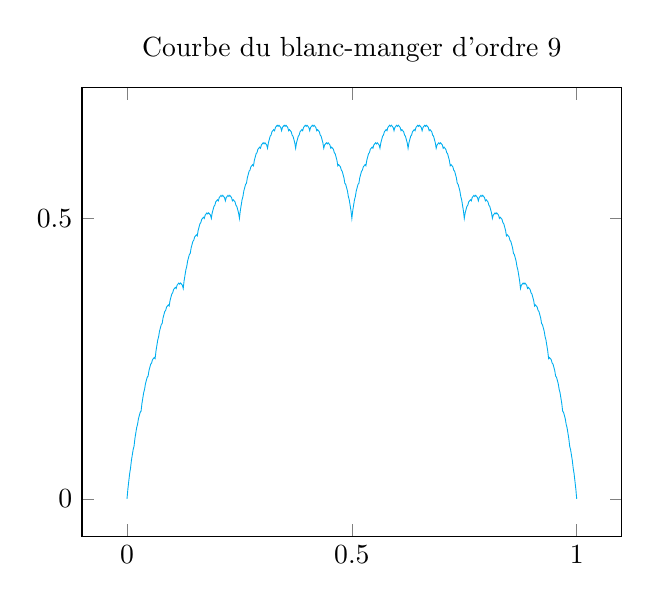
\begin{tikzpicture}

\begin{axis}[
title={Courbe du blanc-manger d'ordre 9},
xtick={0, 1/2, 1}, 
ytick={0, 1/2, 1}
]
\addplot [line width=0.32pt, cyan]
table {%
0 0
0.001953125 0.017578125
0.00390625 0.03125
0.005859375 0.044921875
0.0078125 0.0546875
0.009765625 0.068359375
0.01171875 0.078125
0.013671875 0.087890625
0.015625 0.09375
0.017578125 0.107421875
0.01953125 0.1171875
0.021484375 0.126953125
0.0234375 0.1328125
0.025390625 0.142578125
0.02734375 0.1484375
0.029296875 0.154296875
0.03125 0.15625
0.033203125 0.169921875
0.03515625 0.1796875
0.037109375 0.189453125
0.0390625 0.1953125
0.041015625 0.205078125
0.04296875 0.2109375
0.044921875 0.216796875
0.046875 0.21875
0.048828125 0.228515625
0.05078125 0.234375
0.052734375 0.240234375
0.0546875 0.2421875
0.056640625 0.248046875
0.05859375 0.25
0.060546875 0.251953125
0.0625 0.25
0.064453125 0.263671875
0.06640625 0.2734375
0.068359375 0.283203125
0.0703125 0.2890625
0.072265625 0.298828125
0.07421875 0.3046875
0.076171875 0.310546875
0.078125 0.3125
0.080078125 0.322265625
0.08203125 0.328125
0.083984375 0.333984375
0.0859375 0.3359375
0.087890625 0.341796875
0.08984375 0.34375
0.091796875 0.345703125
0.09375 0.34375
0.095703125 0.353515625
0.09765625 0.359375
0.099609375 0.365234375
0.1015625 0.3671875
0.103515625 0.373046875
0.10546875 0.375
0.107421875 0.376953125
0.109375 0.375
0.111328125 0.380859375
0.11328125 0.3828125
0.115234375 0.384765625
0.1171875 0.3828125
0.119140625 0.384765625
0.12109375 0.3828125
0.123046875 0.380859375
0.125 0.375
0.126953125 0.388671875
0.12890625 0.3984375
0.130859375 0.408203125
0.1328125 0.4140625
0.134765625 0.423828125
0.13671875 0.4296875
0.138671875 0.435546875
0.140625 0.4375
0.142578125 0.447265625
0.14453125 0.453125
0.146484375 0.458984375
0.1484375 0.4609375
0.150390625 0.466796875
0.15234375 0.46875
0.154296875 0.470703125
0.15625 0.46875
0.158203125 0.478515625
0.16015625 0.484375
0.162109375 0.490234375
0.1640625 0.4921875
0.166015625 0.498046875
0.16796875 0.5
0.169921875 0.501953125
0.171875 0.5
0.173828125 0.505859375
0.17578125 0.5078125
0.177734375 0.509765625
0.1796875 0.5078125
0.181640625 0.509765625
0.18359375 0.5078125
0.185546875 0.505859375
0.1875 0.5
0.189453125 0.509765625
0.19140625 0.515625
0.193359375 0.521484375
0.1953125 0.5234375
0.197265625 0.529296875
0.19921875 0.53125
0.201171875 0.533203125
0.203125 0.53125
0.205078125 0.537109375
0.20703125 0.5390625
0.208984375 0.541015625
0.2109375 0.5390625
0.212890625 0.541015625
0.21484375 0.5390625
0.216796875 0.537109375
0.21875 0.53125
0.220703125 0.537109375
0.22265625 0.5390625
0.224609375 0.541015625
0.2265625 0.5390625
0.228515625 0.541015625
0.23046875 0.5390625
0.232421875 0.537109375
0.234375 0.53125
0.236328125 0.533203125
0.23828125 0.53125
0.240234375 0.529296875
0.2421875 0.5234375
0.244140625 0.521484375
0.24609375 0.515625
0.248046875 0.509765625
0.25 0.5
0.251953125 0.513671875
0.25390625 0.5234375
0.255859375 0.533203125
0.2578125 0.5390625
0.259765625 0.548828125
0.26171875 0.5546875
0.263671875 0.560546875
0.265625 0.5625
0.267578125 0.572265625
0.26953125 0.578125
0.271484375 0.583984375
0.2734375 0.5859375
0.275390625 0.591796875
0.27734375 0.59375
0.279296875 0.595703125
0.28125 0.59375
0.283203125 0.603515625
0.28515625 0.609375
0.287109375 0.615234375
0.2890625 0.6171875
0.291015625 0.623046875
0.29296875 0.625
0.294921875 0.626953125
0.296875 0.625
0.298828125 0.630859375
0.30078125 0.6328125
0.302734375 0.634765625
0.3046875 0.6328125
0.306640625 0.634765625
0.30859375 0.6328125
0.310546875 0.630859375
0.3125 0.625
0.314453125 0.634765625
0.31640625 0.640625
0.318359375 0.646484375
0.3203125 0.6484375
0.322265625 0.654296875
0.32421875 0.65625
0.326171875 0.658203125
0.328125 0.65625
0.330078125 0.662109375
0.33203125 0.6640625
0.333984375 0.666015625
0.3359375 0.6640625
0.337890625 0.666015625
0.33984375 0.6640625
0.341796875 0.662109375
0.34375 0.65625
0.345703125 0.662109375
0.34765625 0.6640625
0.349609375 0.666015625
0.3515625 0.6640625
0.353515625 0.666015625
0.35546875 0.6640625
0.357421875 0.662109375
0.359375 0.65625
0.361328125 0.658203125
0.36328125 0.65625
0.365234375 0.654296875
0.3671875 0.6484375
0.369140625 0.646484375
0.37109375 0.640625
0.373046875 0.634765625
0.375 0.625
0.376953125 0.634765625
0.37890625 0.640625
0.380859375 0.646484375
0.3828125 0.6484375
0.384765625 0.654296875
0.38671875 0.65625
0.388671875 0.658203125
0.390625 0.65625
0.392578125 0.662109375
0.39453125 0.6640625
0.396484375 0.666015625
0.3984375 0.6640625
0.400390625 0.666015625
0.40234375 0.6640625
0.404296875 0.662109375
0.40625 0.65625
0.408203125 0.662109375
0.41015625 0.6640625
0.412109375 0.666015625
0.4140625 0.6640625
0.416015625 0.666015625
0.41796875 0.6640625
0.419921875 0.662109375
0.421875 0.65625
0.423828125 0.658203125
0.42578125 0.65625
0.427734375 0.654296875
0.4296875 0.6484375
0.431640625 0.646484375
0.43359375 0.640625
0.435546875 0.634765625
0.4375 0.625
0.439453125 0.630859375
0.44140625 0.6328125
0.443359375 0.634765625
0.4453125 0.6328125
0.447265625 0.634765625
0.44921875 0.6328125
0.451171875 0.630859375
0.453125 0.625
0.455078125 0.626953125
0.45703125 0.625
0.458984375 0.623046875
0.4609375 0.6171875
0.462890625 0.615234375
0.46484375 0.609375
0.466796875 0.603515625
0.46875 0.59375
0.470703125 0.595703125
0.47265625 0.59375
0.474609375 0.591796875
0.4765625 0.5859375
0.478515625 0.583984375
0.48046875 0.578125
0.482421875 0.572265625
0.484375 0.5625
0.486328125 0.560546875
0.48828125 0.5546875
0.490234375 0.548828125
0.4921875 0.5390625
0.494140625 0.533203125
0.49609375 0.5234375
0.498046875 0.513671875
0.5 0.5
0.501953125 0.513671875
0.50390625 0.5234375
0.505859375 0.533203125
0.5078125 0.5390625
0.509765625 0.548828125
0.51171875 0.5546875
0.513671875 0.560546875
0.515625 0.5625
0.517578125 0.572265625
0.51953125 0.578125
0.521484375 0.583984375
0.5234375 0.5859375
0.525390625 0.591796875
0.52734375 0.59375
0.529296875 0.595703125
0.53125 0.59375
0.533203125 0.603515625
0.53515625 0.609375
0.537109375 0.615234375
0.5390625 0.6171875
0.541015625 0.623046875
0.54296875 0.625
0.544921875 0.626953125
0.546875 0.625
0.548828125 0.630859375
0.55078125 0.6328125
0.552734375 0.634765625
0.5546875 0.6328125
0.556640625 0.634765625
0.55859375 0.6328125
0.560546875 0.630859375
0.5625 0.625
0.564453125 0.634765625
0.56640625 0.640625
0.568359375 0.646484375
0.5703125 0.6484375
0.572265625 0.654296875
0.57421875 0.65625
0.576171875 0.658203125
0.578125 0.65625
0.580078125 0.662109375
0.58203125 0.6640625
0.583984375 0.666015625
0.5859375 0.6640625
0.587890625 0.666015625
0.58984375 0.6640625
0.591796875 0.662109375
0.59375 0.65625
0.595703125 0.662109375
0.59765625 0.6640625
0.599609375 0.666015625
0.6015625 0.6640625
0.603515625 0.666015625
0.60546875 0.6640625
0.607421875 0.662109375
0.609375 0.65625
0.611328125 0.658203125
0.61328125 0.65625
0.615234375 0.654296875
0.6171875 0.6484375
0.619140625 0.646484375
0.62109375 0.640625
0.623046875 0.634765625
0.625 0.625
0.626953125 0.634765625
0.62890625 0.640625
0.630859375 0.646484375
0.6328125 0.6484375
0.634765625 0.654296875
0.63671875 0.65625
0.638671875 0.658203125
0.640625 0.65625
0.642578125 0.662109375
0.64453125 0.6640625
0.646484375 0.666015625
0.6484375 0.6640625
0.650390625 0.666015625
0.65234375 0.6640625
0.654296875 0.662109375
0.65625 0.65625
0.658203125 0.662109375
0.66015625 0.6640625
0.662109375 0.666015625
0.6640625 0.6640625
0.666015625 0.666015625
0.66796875 0.6640625
0.669921875 0.662109375
0.671875 0.65625
0.673828125 0.658203125
0.67578125 0.65625
0.677734375 0.654296875
0.6796875 0.6484375
0.681640625 0.646484375
0.68359375 0.640625
0.685546875 0.634765625
0.6875 0.625
0.689453125 0.630859375
0.69140625 0.6328125
0.693359375 0.634765625
0.6953125 0.6328125
0.697265625 0.634765625
0.69921875 0.6328125
0.701171875 0.630859375
0.703125 0.625
0.705078125 0.626953125
0.70703125 0.625
0.708984375 0.623046875
0.7109375 0.6171875
0.712890625 0.615234375
0.71484375 0.609375
0.716796875 0.603515625
0.71875 0.59375
0.720703125 0.595703125
0.72265625 0.59375
0.724609375 0.591796875
0.7265625 0.5859375
0.728515625 0.583984375
0.73046875 0.578125
0.732421875 0.572265625
0.734375 0.5625
0.736328125 0.560546875
0.73828125 0.5546875
0.740234375 0.548828125
0.7421875 0.5390625
0.744140625 0.533203125
0.74609375 0.5234375
0.748046875 0.513671875
0.75 0.5
0.751953125 0.509765625
0.75390625 0.515625
0.755859375 0.521484375
0.7578125 0.5234375
0.759765625 0.529296875
0.76171875 0.53125
0.763671875 0.533203125
0.765625 0.53125
0.767578125 0.537109375
0.76953125 0.5390625
0.771484375 0.541015625
0.7734375 0.5390625
0.775390625 0.541015625
0.77734375 0.5390625
0.779296875 0.537109375
0.78125 0.53125
0.783203125 0.537109375
0.78515625 0.5390625
0.787109375 0.541015625
0.7890625 0.5390625
0.791015625 0.541015625
0.79296875 0.5390625
0.794921875 0.537109375
0.796875 0.53125
0.798828125 0.533203125
0.80078125 0.53125
0.802734375 0.529296875
0.8046875 0.5234375
0.806640625 0.521484375
0.80859375 0.515625
0.810546875 0.509765625
0.8125 0.5
0.814453125 0.505859375
0.81640625 0.5078125
0.818359375 0.509765625
0.8203125 0.5078125
0.822265625 0.509765625
0.82421875 0.5078125
0.826171875 0.505859375
0.828125 0.5
0.830078125 0.501953125
0.83203125 0.5
0.833984375 0.498046875
0.8359375 0.4921875
0.837890625 0.490234375
0.83984375 0.484375
0.841796875 0.478515625
0.84375 0.46875
0.845703125 0.470703125
0.84765625 0.46875
0.849609375 0.466796875
0.8515625 0.4609375
0.853515625 0.458984375
0.85546875 0.453125
0.857421875 0.447265625
0.859375 0.4375
0.861328125 0.435546875
0.86328125 0.4296875
0.865234375 0.423828125
0.8671875 0.4140625
0.869140625 0.408203125
0.87109375 0.3984375
0.873046875 0.388671875
0.875 0.375
0.876953125 0.380859375
0.87890625 0.3828125
0.880859375 0.384765625
0.8828125 0.3828125
0.884765625 0.384765625
0.88671875 0.3828125
0.888671875 0.380859375
0.890625 0.375
0.892578125 0.376953125
0.89453125 0.375
0.896484375 0.373046875
0.8984375 0.3671875
0.900390625 0.365234375
0.90234375 0.359375
0.904296875 0.353515625
0.90625 0.34375
0.908203125 0.345703125
0.91015625 0.34375
0.912109375 0.341796875
0.9140625 0.3359375
0.916015625 0.333984375
0.91796875 0.328125
0.919921875 0.322265625
0.921875 0.3125
0.923828125 0.310546875
0.92578125 0.3046875
0.927734375 0.298828125
0.9296875 0.2890625
0.931640625 0.283203125
0.93359375 0.2734375
0.935546875 0.263671875
0.9375 0.25
0.939453125 0.251953125
0.94140625 0.25
0.943359375 0.248046875
0.9453125 0.2421875
0.947265625 0.240234375
0.94921875 0.234375
0.951171875 0.228515625
0.953125 0.21875
0.955078125 0.216796875
0.95703125 0.2109375
0.958984375 0.205078125
0.9609375 0.1953125
0.962890625 0.189453125
0.96484375 0.1796875
0.966796875 0.169921875
0.96875 0.15625
0.970703125 0.154296875
0.97265625 0.1484375
0.974609375 0.142578125
0.9765625 0.1328125
0.978515625 0.126953125
0.98046875 0.1171875
0.982421875 0.107421875
0.984375 0.09375
0.986328125 0.087890625
0.98828125 0.078125
0.990234375 0.068359375
0.9921875 0.0546875
0.994140625 0.044921875
0.99609375 0.03125
0.998046875 0.017578125
1 0
};
\end{axis}

\end{tikzpicture}

\end{figure}

\begin{defi}{Distance à $\Z$}
    Pour tout $x \in \R$, on définit la fonction $\ll x \gg$ distance de $x$ à $\Z$. 
\end{defi}

\begin{prop}{Expression de $\ll \cdot \gg$}
$$\ll \cdot \gg : x \mapsto \left| x - \left\lfloor x + \frac{1}{2} \right\rfloor \right|$$
\end{prop}

\begin{preuve}
    
\end{preuve}

\begin{defi}{Courbe du blancmanger ou de \textsc{Takagi}}
On définit cette courbe par la fonction
    \begin{alignat*}{2}
        \tau\ :\ [0,1]\ &\longrightarrow\ [0,1]\\
        x\ &\longmapsto\ \sum\limits_{k=0}^\infty \frac{1}{2^k} \ll 2^k x \gg.
    \end{alignat*}
\end{defi}

\subsection{Courbe de \textsc{Bolzano}-\textsc{Lebesgue}}    

\begin{defi}{Courbe de \textsc{Bolzano}-\textsc{Lebesgue}}
    On pose $I \defeq [0, 1]$ et $(f_n)$ la suite de fonctions définie par
    \begin{itemize}
        \item $f_0(x) = x.$
        \item $f_n$ est affine sur $\left[ \frac{k}{3^n}, \frac{k+1}{3^n} \right]$ pour tout $k \in \llbracket 0, 3^n - 1 \rrbracket$.
        \item $f_n$ et $f_{n-1}$ sont égales en $\frac{3k}{3^n}$, $\frac{3k+1}{3^n}$ et $\frac{3k+2}{3^n}$ pour tout $k \in \llbracket 0, 3^n-1 \rrbracket$.
    \end{itemize}
\end{defi}

\subsection{Densité de $F$ dans $E$}

\begin{theo}{}
    $F$ est dense dans $E$ pour la topologie uniforme.
\end{theo}

\begin{preuve}
    \marginnote[0cm]{\url{https://share.miple.co/content/XEZ7y9BayeSN1}}
    Soient $f \in E$ et $W \in F$. La fonction $f - W$ est continue sur $[0, 1]$ donc peut être approchée uniformément par une suite $(A_n)_{n \in \N}$ de fonctions polynomiales définies sur $[0, 1]$ d'après le théorème de \textsc{Weierstrass}. \\
    Pour tout $n \in \N$, notons $B_n \defeq A_n + W$. La fonction $B_n$ est continue et nulle part dérivable puisque si $(B_n)_{n \in \N}$ était dérivable en $x \in [0, 1]$, la fonction $W$ le serait aussi. La suite $(B_n)_{n \in \N}$ est donc une suite de fonctions continues sur $[0,1]$ et nulle part dérivable qui converge uniformément vers la fonction $f$.
\end{preuve}

- \url{http://christophebertault.fr/documents/articles/Article - Une famille nombreuse de fonctions continues partout derivables nulle part.pdf} \\
- lire le paragraphe éponyme dans \cite{contre-exemples} page 350. \\

\section{A rajouter}

\begin{itemize}
    \item Intégrale à paramètre vs. série de fonctions
    \item Développements asymptotiques de sommes de séries de fonctions
\end{itemize}
